\begin{frame}[shrink=10]
\frametitle{John von Neumann}
\begin{center}
\includegraphics[width=0.5\textwidth]{generated/computer/cpu-vonNeumann.pdf}
\phantom{XXXXXXX}
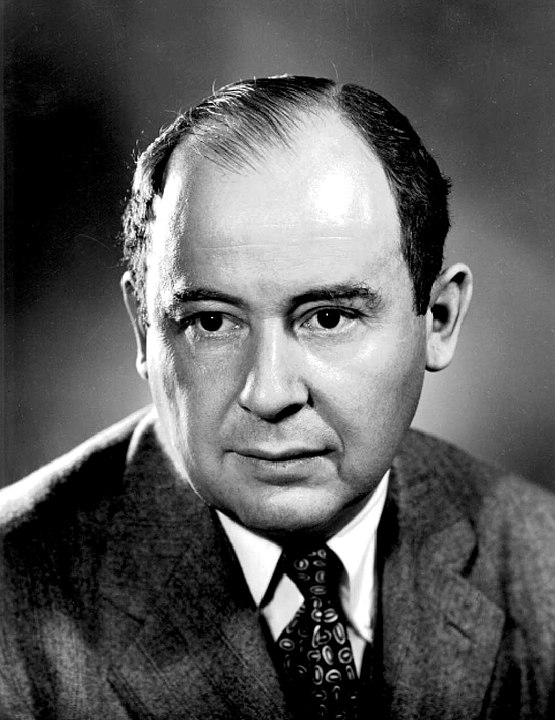
\includegraphics[width=0.15\textwidth]{common/computer/vonNeumann.png}
\end{center}
\begin{itemize}
\item 5 základních jednotek – řídicí jednotka, aritmeticko-logická jednotka, paměť, vstup (vstupní zařízení), výstup (výstupní zařízení)
\item Architektura počítače by neměla být závislá na řešené úloze, měla by umět provádět program uložený v paměti. Program řídí, co počítač vykonává za instrukce a tím jaké dostane výsledky.
\item Program a data jsou uložena ve stejné paměti, složené z buněk (jednotek) stejné velikosti. Oproti tomu Harvardská architektura měla jeden typ paměti pro program a jiný typ paměti pro data.
\item Další instrukce, která se bude vykonávat je uložena v následující buňce paměti (mimo skoků v programu)
\item Instrukce provádějí aritmetické a logické operace, přesuny dat z/do paměti, skoky a větvení programu a speciální řídicí instrukce.
\end{itemize}
\end{frame}


\begin{frame}
\frametitle{Počítač založený na von Neumannově konceptu}

Paměť:
\begin{itemize}
\item von Neumannova architektura používá společnou paměť pro program i data -- to umožňuje například i nahrání programu operačním systémem z disku do paměti a jeho spuštění, vykonávání jako instrukce
\item paměť se skládá z buněk - jednotek, v současné době z bajtů
\end{itemize}

Vstupně výstupní podsystém:
\begin{itemize}
\item Vstupy -- klávesnice, myši, děrné štítky, magnetopáskové jednotky, síťové karty, ...
\item Výstupy -- monitory (grafické karty), tiskárny, plotry, síťové karty, ...
\end{itemize}

Procesor / mikroprocesor:
\begin{itemize}
\item Řídicí jednota (control unit)
\item Registry
\item Aritmeticko-logická jednotka -- ALU
\end{itemize}

\end{frame}

\begin{frame}
\frametitle{Procesor pro von Neumannou koncepci}

Aritmeticko logická jednotka (součást datové cesty):
\begin{itemize}
\item funkce již byly popsané na principech sčítíní, násobení, dělení
\item stejně jako logické oprece a posuny
\item výběr operace multiplexovaný/řízený instrukcí
\end{itemize}

Řídicí jednotka řídí práci a sekvenci této práce. Skládá se z:
\begin{itemize}
\item řídicích hradel -- dekódují instrukce a provádí operace
\item realizace/řízení registrů -- udržují mezivýpočty a stavy výpočtů
\end{itemize}

Registry (součást datové cesty):
\begin{itemize}
\item jsou místa v procesoru, kde se ukládají hodnoty
\item počet bitů registru určuje typ architektury, od 8-mi bitových až po 64-bitové (multimediální regsitry i delší, např. 512 bitů)
\item jsou nejrychlejší pamětí v počítači, HW jsou kontruované naprosto jinak než RAM
\end{itemize}

\end{frame}


\begin{frame}
\frametitle{Nejdůležitější registry procesoru}
\begin{itemize}
\item PC (Program Counter) -- adresa právě prováděné (nebo následující) instrukce
\item IR (Instruction Register) -- obsahje kód prováděné instrukce načtený z paměti
\item Další obvykle přítomné registry
\begin{itemize}
\item GPRs (General purpose registers) -- obecné uživatelské registry, mohou se dělit na data a adresy do paměti, nebo být univerzální
\item SP (Stack Pointer) -- ukazuje na vrchol zásobníku, slouží k organizaci lokálních dat funkcí
\item PSW (Program Status Word) -- definuje v jakém stavu je procesor
\item IM (Interrupt Mask) -- kontrola přerušení
\item FPRs (Floating point registers) -- rozšíření procesoru pro práci s reálnými čísly, případně i vektorové/multimediální registry
\end{itemize}
\end{itemize}
\end{frame}

